\documentclass{article}
\usepackage{german}

\setlength{\emergencystretch}{15pt}

\usepackage{graphicx}

\usepackage{amsmath}

\begin{document}

\section{Herleitung}

\subsection{Methode}
Der einfachheit halbar mit reellen zahlen -> kann auf komplexe übertragen werden
\paragraph{Start}
$z_k^{(i)} = x;z_k^{(i+1)} = y$ in die Weierstraß-Iteration einsetzen 
\begin{equation}
    g(x) = y = x - \frac{p(x)}{\prod_{j=1;j\neq k}^{n} (x-z_j^{(i)})}
\end{equation}
Graph angucken (Beispiel)
\begin{figure}[h]
    \centering
    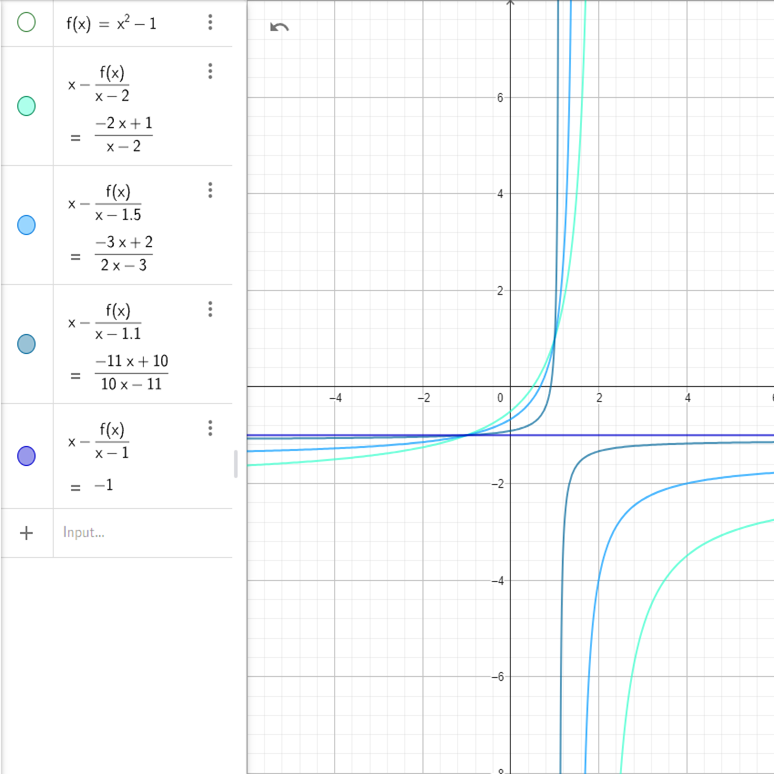
\includegraphics[scale=.6]{BeispielHerleitung.png}
    \caption{Beispiel: $x^2-1$ für die Nullstelle $-1$}
\end{figure}
%-------------------------------------------------------------------------------------------------------------------
\paragraph{?}
Gebrochen rationale Funktion
%-------------------------------------------------------------------------------------------------------------------
\paragraph{waagrechte Asymptote}
Hat waagrechte Asymptote
Sieht man daran:
\begin{align*}
    y &= x - \frac{p(x)}{\prod_{j=1;j\neq k}^{n} (x-z_j^{(i)})} \\
    &= \frac{x}{1} - \frac{\prod_{j=1}^{n} (x-z_j^{(i)})}{\prod_{j=1;j\neq k}^{n} (x-z_j^{(i)})} \\
    &= \frac{x \cdot \prod_{j=1;j\neq k}^{n} (x-z_j^{(i)})}{\prod_{j=1;j\neq k}^{n} (x-z_j^{(i)})} - \frac{\prod_{j=1}^{n} (x-z_j^{(i)})}{\prod_{j=1;j\neq k}^{n} (x-z_j^{(i)})} \\
    &= \frac{x \cdot \prod_{j=1;j\neq k}^{n} (x-z_j^{(i)}) - \prod_{j=1}^{n} (x-z_j^{(i)})}{\prod_{j=1;j\neq k}^{n} (x-z_j^{(i)})} \\
\end{align*}
Da die Polynome im Zähler normiert und vom gleichen Grad sind kann, besitzen beide den Term $x^n$. Werden diese Polynome nun miteinander subtrahiert, ergibt $x^n-x^n$ null. Somit ist der Grad des Differenzpolynoms $n-1$ \\
\begin{equation*}
    y = \frac{\text{Polynom vom Grad }n-1}{\text{Polynom vom Grad }n-1}
\end{equation*}
%-------------------------------------------------------------------------------------------------------------------
\paragraph{Bedeuteung für die Weierstraß-Iteration}
Mit der ersten Iteration wird, falls weit genug von Definitionslücke weg, auf positive oder negative seite gegangen
    Beweis, dass waagrechte Asymptote gleiches vorzeichen wie nullstelle hat
\\
Da waagrechte Asymptote -> Mit nötigem Abstand zu Definitionslücken $|g(x)|<|x|$
-> Methode \glqq entkommt\grqq\space nicht
-> geht, Mit nötigem Abstand zu Definitionslücken $|g(x)|<|x|$, näher an die Nullstelle herran
%-------------------------------------------------------------------------------------------------------------------
\paragraph{verhalten in der nähe der Nullstelle}
$g(x)$ wird immer genauer, wenn die anderen Nullstellen genauer werden
-> alles wird genauer parallel
%-------------------------------------------------------------------------------------------------------------------
\paragraph{verhalten auf der Nullstelle}
$g(z_k) = z_k$ -> Konvergiert -> Nullstelle gefundne
\\
Kann man auch daran sehen:
\begin{align*}
    y &= x - \frac{p(x)}{\prod_{j=1;j\neq k}^{n} (x-z_j)} \\
    &= x - (x-z_k) \\
    &= z_k
\end{align*}
%-------------------------------------------------------------------------------------------------------------------
\paragraph{Außnahmen und Probleme}
Wenn zu nah an Definitionslücke verfälschte Werte
Kann ein Sprung weg sein -> verfälschung aller Werte -> mehr Iterationen benötigt
\\
Manchmal nicht Konvergiert, weil hin und herspringen von nähe von Definitionslücken

\end{document}